\chapter{Исследовательская часть}
\hspace{\parindent}В данном разделе будет проведен сравнительный анализ алгоритмов по времени выполнения в зависимости от количества матриц и их размеров.

\section{Технические характеристики}
\hspace{\parindent}Технические характеристики устройства, на котором выполнялось тестирование представлены далее:

\begin{enumerate}
    \item операционная система: Windows 10 pro;
    \item память: 32 Гб;
    \item процессор: 12h Gen Intel(R) Core(TM) i5-12400 2.50 Ггц.
\end{enumerate}
\hspace{\parindent}Во время замеров компьютер был включен в сеть электропитания и был нагружен только системными программами и программой замеров.
\clearpage

\section{Демонстрация работы программы}
\hspace{\parindent}На рис. \ref{fig:demonstration} представлена демонстрация работы программы. 

\begin{figure}[h]
	\centering
	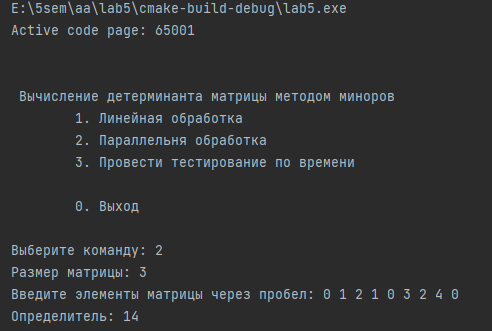
\includegraphics[height=0.4\textheight]{img/ex.png}
	\caption{Демонстрация работы программы}
	\label{fig:demonstration}
\end{figure}

\clearpage
\section{Время выполнения алгоритмов}
\hspace{\parindent}Результаты замеров приведены в таблице \ref{tbl:time}. Время указано в секундах.

\begin{table}[H]
	\begin{center}
		\centering
		\captionsetup{skip=0pt,justification=raggedright,singlelinecheck=off}
		\caption{Результаты замеров по времени}
		\label{tbl:time}
		\begin{tabular}{|r|r|r|}
			\hline
			Размер матрицы & Линейная & Многопоточная\\
			\hline
			1 & 0.0369 & 0.0458 \\
			\hline
			2 & 0.0937 & 0.0952 \\
			\hline
			3 & 1.1308 & 1.0358 \\
			\hline
			4 & 1.7972 & 1.0973 \\
			\hline
			5 & 2.5906 & 1.4571 \\
			\hline
			6 & 3.1332 & 1.8589 \\
			\hline
			7 & 4.1956 & 2.0545 \\
			\hline
			8 & 5.4542 & 2.2654 \\
			\hline
			9 & 6.8004 & 2.7832 \\
			\hline
			10 & 8.0206 & 3.1296 \\
			\hline
		\end{tabular}
	\end{center}
\end{table}

На рис. \ref{fig:measure} представлен графический результат замеров времени работы линейного и многопоточного алгоритма поиска определителя. 

\begin{figure}[h]
	\centering
	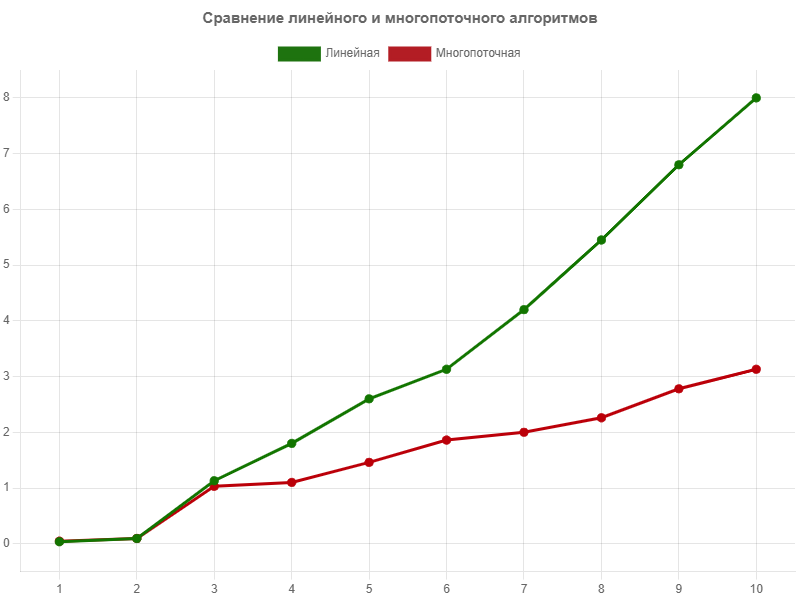
\includegraphics[height=0.4\textheight]{img/measure.png}
	\caption{Сравнение времени работы алгоритмов}
	\label{fig:measure}
\end{figure}